\documentclass[conference]{IEEEtran}
\usepackage{cite}
\usepackage{amsmath,amssymb}
\usepackage{graphicx}
\usepackage{booktabs}
\usepackage{url}
\usepackage{textcomp}
\usepackage{xcolor}
% BasicTeX's minimal install is missing the Courier (psnfss) TFM
% metrics IEEEtran's default typography substitutes \texttt to. Force
% Computer Modern Typewriter instead, which is always present -- pure
% typography fallback, does not change any content.
\renewcommand{\ttdefault}{cmtt}

% Full IEEEtran manuscript/preprint version. SmartGridComm is a strong
% topical fit (privacy/security, data analytics, control/operations),
% but this 10-page full version is not intended to imply compliance
% with a specific conference page limit. Prepare a venue-specific
% condensed submission separately once the target call is selected.

\begin{document}

\title{Evaluating the Value of Topology-Aware Features for Cyber-Physical Grid Monitoring: Detection, Localization, and Real-Time Feasibility}

\author{
\IEEEauthorblockN{Yagiz Sarapli}
\IEEEauthorblockA{
Department of Electrical Engineering and Information Technology\\
TU Dortmund University\\
Dortmund, Germany\\
yagiz.sarapli@tu-dortmund.de}
}

\maketitle

\begin{abstract}
Distinguishing a cyber false-data-injection attack (FDIA) from a legitimate physical disturbance, localizing it, and doing so within a protection-relevant time budget are usually studied separately. We study detection and localization across three networks (a synthetic inverter-dominated 5-bus microgrid and two standard IEEE test systems, 14-bus and 30-bus), and separately profile real-time feasibility on the 5-bus implementation, with a weighted-least-squares (WLS) AC state estimator, to test whether explicit topology-relational features (neighbor- and incident-edge-comparison statistics) help. The evaluation enforces strict separation between relational and non-relational feature sets, uses deployable WLS residuals rather than oracle state, and selects models exclusively on validation data. On this pipeline, explicit topology-relational features show no reproducible benefit at 5-bus or IEEE 14-bus for detection (gaps of $+0.008\pm0.012$ and $-0.003\pm0.013$ against the best non-relational alternative, sign-unstable at both), but a gap positive in all four tested seeds at IEEE 30-bus ($+0.039\pm0.029$). For localization, the pattern inverts: no reproducible benefit at 5-bus or IEEE 30-bus ($-0.007\pm0.016$ and $+0.002\pm0.023$, both sign-unstable), but a gap never negative across the same four seeds at IEEE 14-bus ($+0.023\pm0.021$). Neither effect is statistically confirmed at this seed count -- a 4-seed $t$-based confidence interval crosses zero for both. Profiling the full decision pipeline against a one-cycle (20\,ms at 50\,Hz) budget on a documented Apple-arm64/macOS 15.6.1 environment gives, across two independent $N{=}300$ reruns, 16.2--17.0\,ms median, 16.4--18.2\,ms p95, and 17.0--19.2\,ms p99 latency, while rare solver-tail maxima reach 89.1--92.7\,ms; the detector does not generalize to a completely unseen attack type (0--1.3\% recall, vs.\ 91--100\% when that type is in training).
\end{abstract}

\begin{IEEEkeywords}
false data injection attack, state estimation, cyber-physical systems, attack localization, real-time systems, feature ablation, inverter-based resources
\end{IEEEkeywords}

\section{Introduction}

Modernizing power grids toward higher penetrations of inverter-based resources (PV, battery storage, grid-forming converters) changes the character of protection and monitoring in two ways relevant here. First, inverters provide far less fault current than synchronous generators, which strains protection schemes designed around synchronous-machine fault signatures \cite{liaqat2026protection}. Second, the same measurement infrastructure used for state awareness is now also an attack surface: an adversary who can spoof a subset of sensor readings can attempt a false-data-injection attack (FDIA) against the state estimator that is, by construction, statistically indistinguishable from a legitimate measurement under a residual-based bad-data test \cite{liu2011false}.

Renewable-heavy grid infrastructure specifically is not a hypothetical target: in December 2025, a destructive cyberattack against Poland's energy sector -- corrupted firmware forced into endless restart cycles across roughly 30 wind and solar farms and a heat-and-power plant, during a cold-weather period, attributed to infrastructure overlapping with the Dragonfly/Static Tundra threat actor -- was contained before it caused a blackout affecting an estimated 500{,}000 people \cite{certpolska2026followup}. That incident was an OT/firmware-integrity attack rather than a state-estimation FDIA specifically, but it establishes the same operational stakes this paper's threat model targets: an operator or automated scheme facing a live control-plane anomaly, under real time pressure, in exactly this class of infrastructure.

A control-room operator, or an automated protection scheme, therefore faces a three-part problem for any anomalous reading: \emph{is this a cyberattack or a physical event}, \emph{where is it}, and -- if it is to inform a protective action rather than only a post-hoc forensic one -- \emph{can a decision be reached inside a protection-relevant time budget}. These three questions are usually studied separately. A large FDIA-detection literature (Section~\ref{sec:related}) asks the first question, typically evaluated offline against a fixed dataset. A smaller attack-localization literature asks the second. Real-time feasibility is addressed by a much smaller, very recent body of work -- notably a 2026 benchmark \cite{abukhousa2026latency} that found deep classifiers for this exact joint task are individually fast (sub-15\,ms) but the measured end-to-end pipeline is not (50--90\,ms), calling this ``a critical gap between algorithmic capability and protection-grade deployment'' and recommending hardware acceleration. A separate, popular line of work asks whether giving a detector explicit \emph{topology} -- not just raw sensor residuals, but how each meter's reading compares to its electrical neighbors -- improves on any of this; that question is this paper's own starting point, and its central subject.

This paper studies detection and localization within a common evaluation framework across three networks, and separately profiles real-time feasibility on the 5-bus implementation. The evaluation framework enforces strict separation between relational and non-relational feature sets, uses deployable WLS residuals rather than oracle state, and selects models exclusively on validation data. We independently reproduce the qualitative pipeline-latency finding of concurrent work \cite{abukhousa2026latency} (fast classifiers embedded in a slow end-to-end pipeline) and localize the actual bottleneck: not the classifier, not the state estimator's Newton-type iteration count, but a measurement-table object being rebuilt from scratch through a general-purpose element-creation API every cycle, when its structure never changes -- fixing that one thing accounts for most of the gap closed.

\subsection{Contributions}
\begin{itemize}
\item A task- and network-specific result across three networks: explicit topology-relational features show no reproducible detection benefit at 5-bus or IEEE 14-bus, but a gap positive in all four tested seeds at IEEE 30-bus; for localization, the pattern inverts -- no reproducible benefit at 5-bus or IEEE 30-bus, but a gap never negative across the same four seeds at IEEE 14-bus (Section~\ref{sec:results1}, Section~\ref{sec:scale}; neither effect is statistically confirmed at this seed count) -- together with a structural, quantitative redundancy analysis that rules out one natural explanation for why the two standard IEEE systems disagree with the custom microgrid.
\item A root-cause profiling methodology for the ``fast model, slow pipeline'' gap identified in prior work, and a demonstrated fix that closes most of it without hardware acceleration (Section~\ref{sec:latency}).
\item A further explicit negative result reported as a scope condition rather than omitted: no zero-day attack-type generalization (Section~\ref{sec:zeroday}).
\end{itemize}

\section{Related Work}
\label{sec:related}

\subsection{Foundational FDIA and Stealth Constructions}
The FDIA threat model used throughout this paper -- an attacker with knowledge of the network model constructing a measurement perturbation that leaves the WLS residual unchanged -- follows Liu, Ning \& Reiter's foundational construction \cite{liu2011false} and its AC-consistent extensions \cite{anwar2016modeling}. A growing subline constructs such attacks with \emph{less} attacker knowledge than the original construction assumes: without line parameters \cite{du2021targeted}, or fully ``blind'' to topology using generative or physics-informed models \cite{zhao2025blind,falas2026learning} -- all harder threat models than the one used here and natural next stress conditions for the attack generator used in this study. In the opposite direction, low-magnitude attacks close to the sensor noise floor -- the specific regime Section~\ref{sec:results1}'s hardened attack magnitude targets -- have their own dedicated detection literature \cite{li2026physically}, worth comparing against directly in future work.

\subsection{Deep-Learning FDIA Detection}
A substantial literature applies CNN/LSTM/transfer-learning architectures to FDIA detection \cite{niu2018dynamic,li2021adversarial,xu2021detecting}, generally evaluated as a binary classification task on a fixed attack distribution. The \texttt{residual\_only} and \texttt{prior\_only} baselines used here sit in this tradition; this paper's contribution is isolating what \emph{explicit topology-relational} features specifically add beyond a fair combination of the two, under a stress-tested (not default-easy) attack distribution, and under features and model-selection procedures that are actually deployable rather than built with access to information a real detector would not have.

\subsection{Topology-Aware / Graph-Based State Estimation and Detection}
The closest published framing to this paper's central question is topology-aware graph neural network (GNN) based state estimation \cite{moshtagh2025topology,moshtagh2022timesync,suri2025powergnn,yaniv2026robust}, which use graph convolution/attention to exploit network structure. Prior work presents a mixed picture. \cite{moshtagh2025topology} and an earlier, closely related study by an overlapping author group \cite{moshtagh2022timesync} compare their GNN against a same-feature ``regular'' DNN baseline (identical PMU-derived node features, no adjacency matrix), providing a correctly scoped topology ablation; \cite{suri2025powergnn}'s non-graph baseline, by contrast, does not clearly document an input-matched comparison. We therefore do \emph{not} claim that topology ablation is generally absent from the GNN-for-power-systems literature. The contribution here is narrower: a same-architecture, same-feature comparison (GNN vs.\ DNN, as in \cite{moshtagh2025topology,moshtagh2022timesync}) checks whether a different \emph{model} benefits from topology, but it does not by itself test how the non-topological feature \emph{set} is constructed or whether all inputs are deployable before model training -- safeguards that are explicit in Section~\ref{sec:method}. Section~\ref{sec:results1}'s out-of-fold linear-redundancy check is offered as a second, complementary, and considerably cheaper pre-check for the feature-leakage variant of this failure mode: verifiable on the feature matrix alone, before training any model, topology-aware or not.

\subsection{Attack/Event Localization}
Localization work spans capsule networks for load-altering (not FDIA) attacks evaluated across 14/39/57-bus systems \cite{jahangir2022localizing}, moving-target-defense-assisted localization \cite{chen2022localization}, and online detection-plus-localization schemes \cite{li2021online}. The cited localization studies do not explicitly document sensitivity to network topology/meshedness or an ablation of relational features against a matched non-relational baseline, which is the comparison examined in Sections~\ref{sec:results1} and \ref{sec:scale}.

\subsection{Real-Time / Latency-Aware Classification}
\cite{abukhousa2026latency} is the direct comparison point for Section~\ref{sec:latency} of this paper -- it independently measures the same qualitative gap (fast model, slow pipeline) on a different, larger testbed using an industrial electromagnetic-transient (EMT) simulator, and calls for hardware acceleration where this paper instead finds and fixes a software-level cause for a comparable fraction of the gap.

\subsection{Zero-Day / Unseen-Attack Generalization}
The general (non-power-specific) intrusion-detection literature widely reports that supervised detectors trained on known attack families do not reliably generalize to unseen ones; a verified, quantitative comparison specific to the power-systems FDIA literature remains an open point for future work.

\subsection{Field-Wide Self-Assessment of Adjacent Gaps}
A 2025 scoping review of ML applications in power-system protection \cite{oelhaf2025scoping} independently reports, at the level of the field rather than any single paper, two gaps this paper runs into directly: most reviewed studies do not discuss computational latency/real-time constraints at all (Section~\ref{sec:latency}), and cross-topology generalization is essentially untested field-wide -- reviewed work concentrates on fixed IEEE 14/30/39-bus evaluations with no cross-topology testing (Section~\ref{sec:scale}). This positions those sections as addressing gaps the field has already flagged in itself, not problems specific to this study's testbed.

\section{Testbed and Methodology}
\label{sec:method}

\subsection{Network}
A 5-bus, 0.4\,kV synthetic microgrid built in \texttt{pandapower}: point of common coupling, a PV bus modeled as a steady-state grid-following (GFL) power injection, a BESS bus modeled as a steady-state grid-forming (GFM) power injection, and two load buses, connected by 4 lines. Both are static \texttt{sgen} operating-point injections, not dynamic converter-control models -- no droop control or virtual inertia is simulated; the GFL/GFM labels describe each device's intended role in the microgrid, not modeled control dynamics. \texttt{net.f\_hz = 50.0} (verified from the model object, not assumed -- this fixes the one-cycle protection-relevant computational target below to 20\,ms).

\subsection{State Estimation}
Weighted least squares (WLS) AC state estimation via \texttt{pandapower.estimation.estimate}, with 23 measurements per cycle: voltage magnitude, and P/Q injection, at all 5 buses, plus P/Q from-side flow on all 4 lines -- the same model-driven/data-driven/hybrid-driven taxonomy of state estimation under measurement anomalies surveyed in \cite{lin2026state} implicitly underlies this paper's own \texttt{residual\_only}/\texttt{prior\_only}/\texttt{topology\_fusion} split. All ``residual'' features throughout this paper (5-bus, IEEE 14-bus, IEEE 30-bus alike) are the standard, deployable normalized measurement residual $(z - h(\hat{x}))/\sigma$ computed from the WLS solution -- never a comparison to a ground-truth state a real detector could not observe.

\subsection{Threat Model}
Two synthetic attack families, both targeting a randomly chosen load bus per scenario:
\begin{itemize}
\item \emph{Naive}: a single voltage-magnitude sensor is spoofed by a fixed-range random offset.
\item \emph{Model-consistent (``stealth'') FDIA}: following the Liu--Ning--Reiter construction adapted to the AC case, the true state is perturbed at the target bus and the corresponding measurement-space attack vector $a = h(x_{\text{attack}}) - h(x_{\text{true}})$ is computed exactly, so the attack is, by construction, invisible to the chi-square residual test.
\end{itemize}
A benign hard-negative physical load disturbance (a 25--70\% load step at a randomly chosen bus) is included specifically to be confusable with an attack in raw residual terms.

\subsection{Prior Construction}
Every replication starts from one randomly sampled base operating point (a load/PV level, shared unmodified across that replication's 4 scenarios). Before any attack or physical disturbance is applied to build the ``true'' network for a given scenario, an independent copy of that same base operating point has its load values perturbed by a fresh, independently drawn forecast error ($\mathcal{N}(0, 2.5\%)$ per load at 5-bus, clipped to $\pm6\%$; $\mathcal{N}(0, 5\%)$ at IEEE 14-bus/30-bus, a cross-network noise-model difference documented as a limitation below) and is solved through its own, separate AC power flow -- this perturbed-and-solved copy is the ``prior.'' \texttt{prior\_only} features are the deviation between the WLS state estimate (computed from the scenario's actual, possibly-attacked measurements) and this prior's own voltage/angle solution. Critically, the prior is constructed \emph{before}, and entirely independently of, whichever scenario (clean, naive attack, stealth attack, physical disturbance) that replication's true network becomes -- it never sees the true or attacked state, only an independently-perturbed forecast of the same nominal base point. This is what lets stealth attacks, invisible in residual space by construction, become visible at all: the attack is only tuned to be consistent with the WLS residual test, not with an estimate the defender never let it see.

\subsection{Feature Sets}
Four feature sets are compared. \texttt{residual\_only}: conventional WLS measurement residuals. \texttt{prior\_only}: the prior-deviation features defined above. \texttt{residual\_plus\_prior}: the two combined, with no relational or structural information at all -- the topology-free ablation. \texttt{topology\_fusion}: \texttt{residual\_plus\_prior} plus explicit relational features describing each bus relative to its network neighbors (local-minus-neighbor innovation/residual, incident-edge aggregates); no static structural metadata (node degree, device role) beyond that, since neither is a scenario-specific neighbor comparison and both risk leaking attack-target eligibility (the attack generator above only ever targets load buses). To preserve the intended ablation, non-relational baselines exclude all relational columns, and static node-degree/device-role metadata is excluded from every feature set because it could encode attack-target eligibility when attacks are restricted to load buses.

\subsection{Models and Evaluation}
LogisticRegression, RandomForest, and HistGradientBoosting classifiers are compared with replication-group-safe 70/15/15 train/validation/test splits and group-aware bootstrap confidence intervals. Model selection uses the validation split exclusively: each candidate model is scored on validation, the best-scoring model per feature set is selected, and only that model's (until then unseen) test-set score is reported.

\subsection{Sample-Size Terminology}
A \emph{replication} is one independently sampled base operating point (load level, forecast draw); each replication produces exactly 4 \emph{scenarios} -- one clean, one naive-attack, one stealth-attack, one physical-disturbance -- so $N$ replications yield $4N$ scenarios in total. The 70/15/15 split is applied at the replication level (never at the scenario level, to keep the 4 matched scenarios from one replication from leaking across train/test), so the resulting \emph{test-scenario count} is $0.15N \times 4$, and the \emph{cyber test-scenario count} used for localization (only the 2 attack scenario types have a real target bus) is half of that. Concretely: the headline 5-bus result uses $N{=}500$ replications $\rightarrow$ 2000 scenarios $\rightarrow$ $\approx$300 test scenarios; Section~\ref{sec:scale}'s IEEE 14-bus/30-bus results use the same $N{=}500$ replications $\rightarrow$ 300 test scenarios for detection, 150 for localization, at both networks. Wherever this paper states ``$n{=}X$'' without qualification, $X$ is the resulting test-scenario count, not the replication count.

\section{Results I: The Topology-Fusion Advantage Does Not Survive Its Own Ablation, at Either Task}
\label{sec:results1}

Attack magnitude is hardened roughly $3\times$ toward the sensor noise floor, relative to the naive detection regime a first pass would produce, and evaluated at $n{=}300$ test scenarios (Section~\ref{sec:method}). \texttt{prior\_only} alone is missing residual information that \texttt{topology\_fusion} has access to, so a comparison against \texttt{prior\_only} specifically cannot, by construction, distinguish ``topology helped'' from ``having residual information at all helped''; the fair comparison is against the topology-free \texttt{residual\_plus\_prior} ablation instead.

\subsection{Primary Ablation}
Table~\ref{tab:ablation} compares \texttt{topology\_fusion} against \texttt{residual\_plus\_prior} (Section~\ref{sec:method}), for the primary seed and both stress conditions.

\begin{table}[t]
\centering
\caption{Topology\_fusion vs.\ the corrected, topology-free ablation (best validation-selected model per cell; 5-bus, $n{=}300$ detection / $n{=}150$ cyber-only localization test scenarios)}
\label{tab:ablation}
\begin{tabular}{@{}lcccc@{}}
\toprule
 & \multicolumn{2}{c}{Detection (bal.\ acc.)} & \multicolumn{2}{c}{Localization (top-1)} \\
Condition & topo.\ fusion & res.+prior & topo.\ fusion & res.+prior \\
\midrule
Hard & 0.950 & 0.937 & 0.967 & 0.967 \\
Harder (+2$\times$ noise) & 0.950 & 0.947 & 0.960 & 0.967 \\
\bottomrule
\end{tabular}
\end{table}

Detection shows a small edge for \texttt{topology\_fusion} at this one seed, in both conditions ($+0.013$ Hard, $+0.003$ Harder); localization is an exact tie under Hard and a small edge for \texttt{residual\_plus\_prior} under Harder ($-0.007$). Neither column is bolded here -- a single seed's small, direction-inconsistent gap is not evidence of a real winner, and the four-seed replication directly below (which includes this same seed) is the test that actually matters. For reference, both feature sets still comfortably beat \texttt{prior\_only} alone (0.860--0.870 detection, 0.687--0.693 localization) and \texttt{residual\_only} alone (0.700 detection, 0.547 localization) -- the gain over either single baseline is large; it is simply not a topology effect.

\begin{figure}[t]
\centering
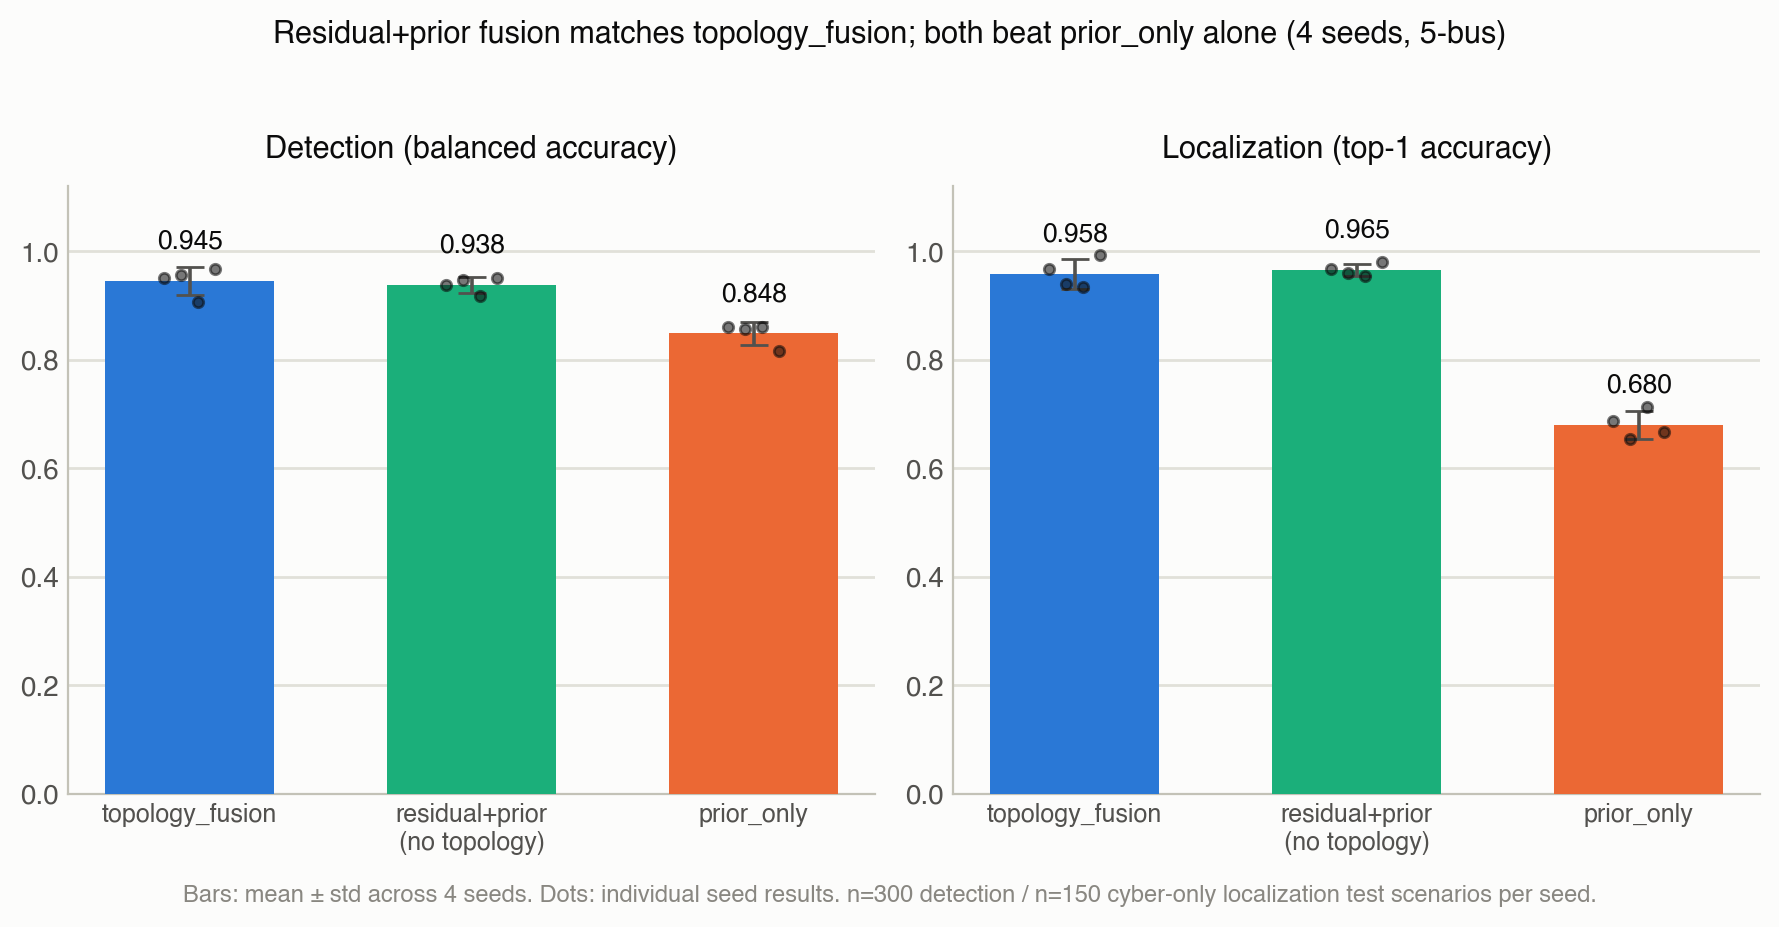
\includegraphics[width=\columnwidth]{paper_fig1_multiseed_advantage.png}
\caption{Topology fusion vs.\ the topology-free residual+prior ablation and the prior-only baseline across four independent random seeds (5-bus, hard attack magnitude). Bars show mean $\pm$ standard deviation; dots show individual seed results. $n{=}300$ detection / $n{=}150$ cyber-only localization test scenarios per seed.}
\label{fig:multiseed}
\end{figure}

\subsection{Multi-Seed Replication}
Figure~\ref{fig:multiseed} summarizes the result. Repeating full data generation and evaluation for four independent seeds, with localization training restricted to cyber-scenario nodes only (matching the convention used at IEEE 14-bus/30-bus, Section~\ref{sec:scale}), gives a \texttt{topology\_fusion}-vs-\texttt{residual\_plus\_prior} detection gap of $+0.008\pm0.012$ (range $-0.010$ to $+0.017$) and a localization gap of $-0.007\pm0.016$ (range $-0.020$ to $+0.013$, including one exact tie): both cross zero and change sign seed to seed, consistent with sampling variability around a near-zero effect in either direction, on either task.

\subsection{Redundancy Diagnostic}
Why would explicit neighbor-comparison features add nothing, given they are computed from genuinely different information -- each bus's residual/innovation relative to its neighbors, not just its own? On this fixed, small (5-bus, 4-line) topology, the result is consistent with high linear recoverability of the relational features from the local feature set. Predicting each of the 65 relational columns from \texttt{residual\_plus\_prior} alone, with 5-fold cross-validated ridge regression, gives a mean out-of-fold $R^2$ of 0.956 (median 1.000, minimum 0.613, 90.8\% of columns above 0.8): a neighbor-mean or incident-edge aggregate over a fixed, small neighbor set is, on a network this size, close to an affine function of the same per-bus values \texttt{residual\_plus\_prior} already provides in full. A sufficiently flexible classifier (HistGradientBoosting, the best model throughout) may therefore reconstruct much of that relational information internally without ever being given it explicitly, which is exactly consistent with Table~\ref{tab:ablation}'s near-ties on both tasks. This explanation is specific to a fixed, small topology, and does not by itself predict what happens at larger, standard networks (Section~\ref{sec:scale}), where an unrelated, size-agnostic feature design is used instead -- reduced recoverability of relational features from local information remains one possible condition under which explicit topology-awareness might help; Section~\ref{sec:scale} tests whether such benefits appear on larger networks, while the Discussion examines whether reduced redundancy explains the observed pattern.

\section{Results II: Real-Time Feasibility -- Diagnosing and Fixing the Gap}
\label{sec:latency}

Following \cite{abukhousa2026latency}'s finding that fast classifiers can still sit inside a slow end-to-end pipeline, we measured the full per-cycle decision pipeline (state estimation $\rightarrow$ feature computation $\rightarrow$ classification) against a one-cycle (20\,ms at the network's confirmed 50\,Hz) protection-relevant computational target -- not a claim that every protective relaying function requires exactly this latency, but the natural reference point for a per-cycle decision loop -- with one-time network/model setup excluded, matching how a deployed scheme would actually operate.

\subsection{Initial Measurement}
Median 42.98\,ms, $2.15\times$ over budget, using the original pipeline (RandomForest classifier, \texttt{tolerance=1e-7}, \texttt{maximum\_iterations=40}, flat state-estimator initialization every cycle).

\subsection{Warm-Start Test}
Warm-starting the state estimator from the previous cycle's converged solution produced only a $1.06\times$ speedup (37.14\,ms), ruling out ``far from the solution'' as the dominant cost.

\subsection{Profiling}
Splitting the state-estimation call into its constituent steps showed the measurement-submission step cost 19.9\,ms -- essentially the same as the estimator's own solve (19.4\,ms). An ablation on \texttt{maximum\_iterations} (40 $\rightarrow$ 5: no speed change; 40 $\rightarrow$ 3: convergence failure in 19/20 trials) showed the true iteration requirement is roughly 4--5 steps regardless of the 40-iteration cap, ruling out iteration count as the estimator-side cost driver.

\subsection{Measurement-Update Optimization}
The measurement table was being rebuilt from scratch every cycle via a general-purpose element-creation API, called once per channel in a Python loop -- even though the table's structure is identical every cycle; only the values change. Replacing this with a one-time table construction followed by an in-place overwrite of the value column each cycle gave a $1158\times$ speedup on this sub-step (19.4\,ms $\rightarrow$ 0.017\,ms), verified to produce a bit-identical state-estimation result (max difference 0.0).

\begin{figure}[t]
\centering
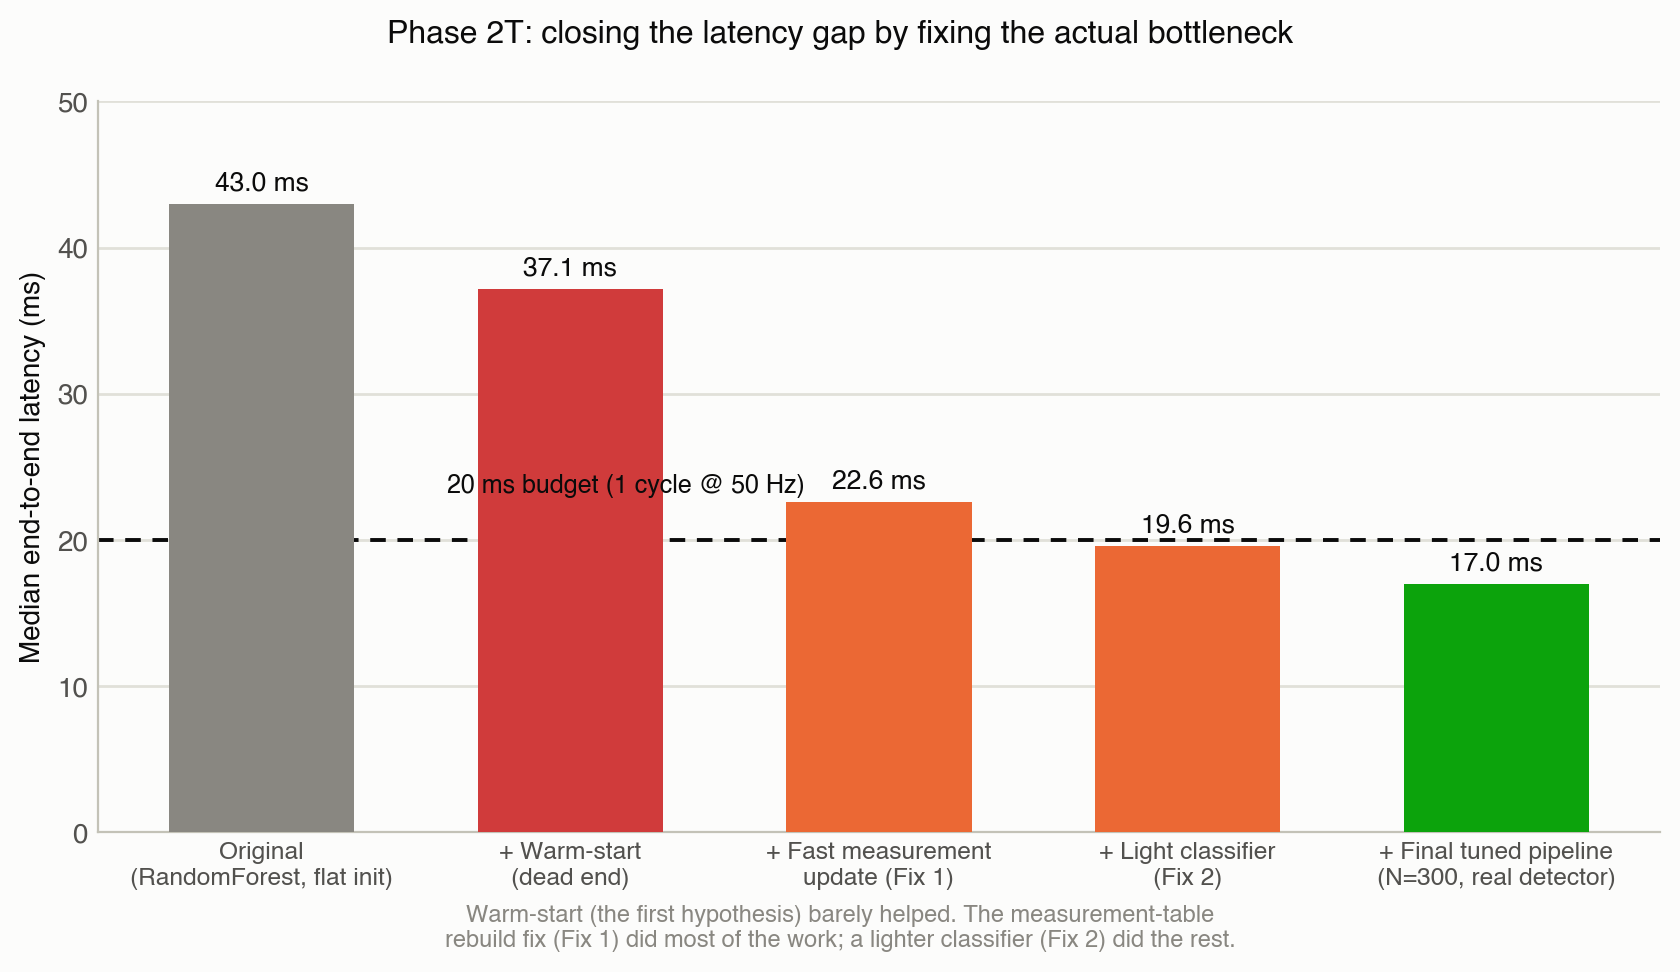
\includegraphics[width=\columnwidth]{paper_fig2_latency_waterfall.png}
\caption{End-to-end latency after successive pipeline optimizations. In-place measurement updates account for most of the reduction; the lighter classifier provides a smaller additional improvement.}
\label{fig:latency}
\end{figure}

\subsection{Final Benchmark}
With a lighter classifier (LogisticRegression, competitive with RandomForest per Section~\ref{sec:results1}'s accuracy results and faster at inference), two independent $N{=}300$ reruns on the same documented environment, both with 0 convergence failures, give 16.155--17.015\,ms median, 16.429--18.211\,ms p95, 16.952--19.190\,ms p99, and 89.067--92.657\,ms max end-to-end latency (Fig.~\ref{fig:latency} shows the most recent run). Median, p95, and p99 remain within the 20\,ms computational budget in both reruns, while the maximum exceeds it in both. Across the same two reruns, stage medians are 15.855--16.664\,ms for WLS state estimation, 0.050--0.057\,ms for post-estimation residual/innovation calculation, 0.083--0.088\,ms for feature computation, 0.0068--0.0076\,ms for array assembly, and 0.160--0.200\,ms for model inference; the WLS solve therefore dominates the budget. The benchmark environment is Apple arm64 running macOS 15.6.1 with Python 3.12.4, pandapower 2.14.10, NumPy 1.26.4, pandas 2.2.2, and scikit-learn 1.4.2. This benchmark uses its own, separately implemented 35-feature representation (7 local-plus-neighbor statistics per bus $\times$ 5 buses) built for the timing measurement specifically, not \texttt{topology\_fusion} or \texttt{residual\_plus\_prior} verbatim; feature computation is a small fraction of the total either way, so the exact feature set used for classification is a second-order cost driver. The classifier is trained on 150 real warm-up scenarios generated through the same simulated pipeline (83 attack, 67 clean; training balanced accuracy 1.000), and the residual/innovation features use the same deployable quantities as everywhere else in this paper; the timer covers all five pipeline stages end to end (state estimation, post-estimation residual/innovation calculation, feature computation, array assembly, inference), so the headline numbers above are the true total, nothing excluded.

\subsection{Positioning}
\cite{abukhousa2026latency} measures the same category of gap (sub-15\,ms classification embedded in 50--90\,ms pipelines) on an industrial-grade EMT simulator and recommends hardware acceleration. This paper's finding -- that a large fraction of a comparable gap traced to avoidable software overhead rather than model inference -- suggests pipeline profiling, not only hardware acceleration, deserves consideration first. A second, independent data point supports the ``classifier inference itself is cheap'' half of this argument: a knowledge-distilled LightGBM detector for virtualized microgrids reports 54--67\,ms per 1000 samples ($\sim$0.06\,ms/sample) for inference alone \cite{ogiesoba2026cyberattack} -- the same order of magnitude as this paper's own model-inference sub-step ($\sim$0.16--0.20\,ms/sample), and far below this paper's state-estimation sub-step ($\sim$15.9--16.7\,ms/sample). Both results point the same way: once a classifier is lightened, the remaining latency budget is spent upstream of the model, not in it.

\section{Results III: The Advantage Does Not Extrapolate to Unseen Attack Types}
\label{sec:zeroday}

To test whether Section~\ref{sec:results1}'s detector generalizes beyond the two attack families it was trained on (as opposed to merely discriminating them well), we trained HistGradientBoosting -- with the same tuned hyperparameters used as the reported 5-bus detector elsewhere in this paper -- with one entire attack family withheld from training and validation, then measured recall on exactly that withheld family, evaluated against the standard test split under a symmetric protocol (the held-out and seen-in-training conditions are compared on the same kind of row) (Table~\ref{tab:zeroday}, Fig.~\ref{fig:zeroday}). Run for both \texttt{topology\_fusion} and the topology-free \texttt{residual\_plus\_prior} ablation, to check directly whether the collapse below is specific to one feature set or, as Section~\ref{sec:results1}'s in-distribution finding would predict, behaviorally identical for both.

\begin{table}[t]
\centering
\caption{Recall on a withheld vs.\ trained-on attack type ($n{=}75$ test scenarios per cell, both conditions)}
\label{tab:zeroday}
\footnotesize
\begin{tabular}{@{}llcc@{}}
\toprule
Attack type & Features & Withheld & In training \\
\midrule
Naive corruption & topo.\ fusion & 0.000 & 0.907 \\
Naive corruption & res.+prior & 0.000 & 0.907 \\
Stealth FDIA & topo.\ fusion & 0.013 & 1.000 \\
Stealth FDIA & res.+prior & 0.013 & 1.000 \\
\bottomrule
\end{tabular}
\end{table}

\begin{figure}[t]
\centering
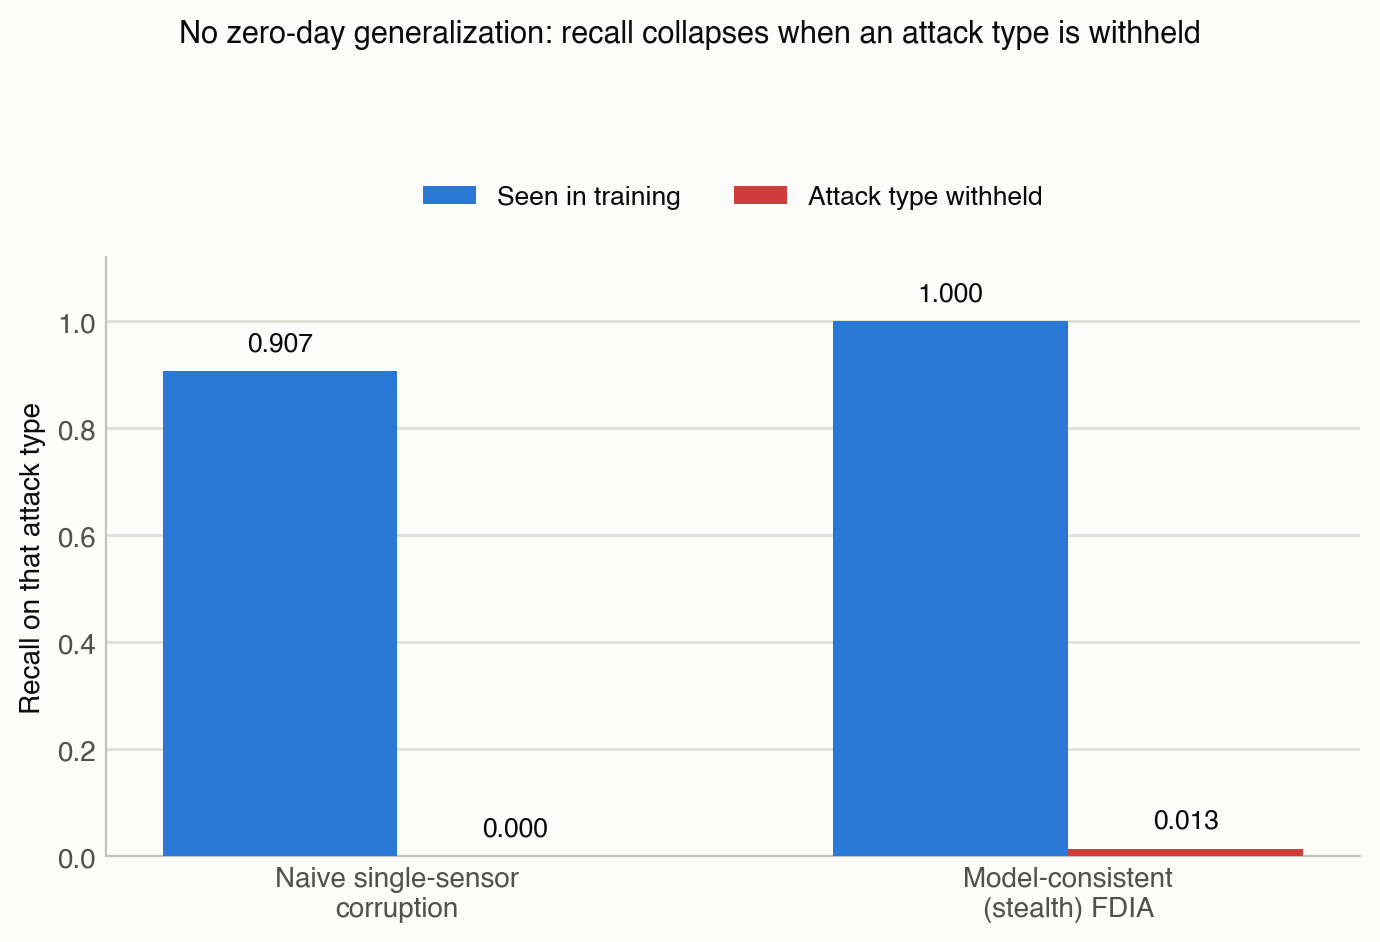
\includegraphics[width=\columnwidth]{paper_fig3_zeroday_generalization.png}
\caption{Recall for attack types represented in training versus withheld from training (topology fusion shown; residual+prior is behaviorally identical, Table~\ref{tab:zeroday}).}
\label{fig:zeroday}
\end{figure}

The detector recognizes the statistical signature of attack types represented in its training data -- including the stealthy one, very well -- but does not extrapolate to a mechanism it has not seen, and this holds identically whether or not topology-relational features are included: the two feature sets are indistinguishable on every cell of Table~\ref{tab:zeroday}, confirming Section~\ref{sec:results1}'s prediction that they are behaviorally interchangeable, here for a question -- generalization to an unseen mechanism -- that has nothing to do with topology specifically. We report this as a hard scope limit on any deployment claim built on Section~\ref{sec:results1}'s results: within this study's two-family attack taxonomy, this is a complete absence of zero-day capability, not a partial one, for either feature set. This complements, from the opposite direction, a related generalization gap documented in the fault-classification literature: an XGBoost-based classifier trained and evaluated on the \emph{same} distribution still drops from 96.8\% (synthetic data) to 85.2\% (physical data) \cite{senyuk2025bulk} -- i.e., even without an unseen attack \emph{type}, a synthetic-to-real distribution shift alone costs over 11 points. Between that gap and this paper's own result, generalization -- of any kind -- looks like the open problem for this class of detector, not an edge case. A deployment-aware zero-day evaluation in the adjacent EV/V2X charging-infrastructure domain \cite{sakr2026explainable} is a useful methodological reference for what a more rigorous version of Section~\ref{sec:zeroday}'s test could look like.

\section{Results IV: Cross-Network Evaluation Reveals Task- and Network-Specific Effects}
\label{sec:scale}

Everything in Sections~\ref{sec:results1}--\ref{sec:zeroday} uses the custom 5-bus microgrid. We separately tested whether explicit topology-relational features help at a larger, standard scale, using a completely independent, size-agnostic feature-engineering design.

\subsection{Test-System Selection}
IEEE 14-bus and IEEE 30-bus were selected because their \texttt{pandapower} bus indexing maps directly to the internal power-flow representation used by the evaluation pipeline (confirmed directly: \texttt{net.bus} count matches the internal power-flow-case bus count for both), and they are, independently, among the most commonly used benchmarks in the power-system state-estimation/FDIA literature specifically.

\subsection{Cross-Network Method}
All WLS/measurement/attack machinery is network-size-agnostic by construction and was reused unmodified. The original fixed per-bus feature columns do not generalize past 5 buses and were replaced with a size-agnostic design: global summary statistics of the residual/innovation arrays, plus, for localization, a trained per-node classifier ranking every bus's probability of being the attack target. This feature design is implemented separately from Section~\ref{sec:method}'s but applies the same safeguards: the residual feature is the deployable measurement residual $z - h(\hat{x})$ (never the simulator's hidden ground-truth state), model selection is validation-based rather than test-set-based, non-relational baselines exclude relational columns, and \texttt{topology\_fusion} excludes static structural metadata such as node degree, which could otherwise act as a target-eligibility prior because attacks are restricted to load buses. All numbers below are from this corrected pipeline, re-run in full at $N{=}500$ replications, four seeds, at both networks.

\begin{table}[t]
\centering
\caption{5-bus vs.\ IEEE 14-bus vs.\ IEEE 30-bus, all 4-seed means, at matched test-set sizes ($n{=}300$ detection / $n{=}150$ cyber-only localization scenarios per network)}
\label{tab:scale}
\footnotesize
\begin{tabular}{@{}lcccc@{}}
\toprule
 & topo. & res.+prior & prior & res. \\
\midrule
Det., 5-bus & 0.945 & 0.938 & 0.848 & 0.682 \\
Det., IEEE-14 & 0.870 & 0.873 & 0.700 & 0.656 \\
Det., IEEE-30 & 0.871 & 0.832 & 0.672 & 0.653 \\
Loc., 5-bus & 0.958 & 0.965 & 0.680 & 0.548 \\
Loc., IEEE-14 & 0.918 & 0.895 & 0.528 & 0.447 \\
Loc., IEEE-30 & 0.910 & 0.908 & 0.515 & 0.427 \\
\bottomrule
\end{tabular}

\smallskip
\footnotesize Per-seed gap direction and uncertainty are reported separately in Section~\ref{sec:results1} and Tables~\ref{tab:ieee14seeds}--\ref{tab:ieee30seeds}; no cell is emphasized as a confirmed winner.
\end{table}

\begin{figure}[t]
\centering
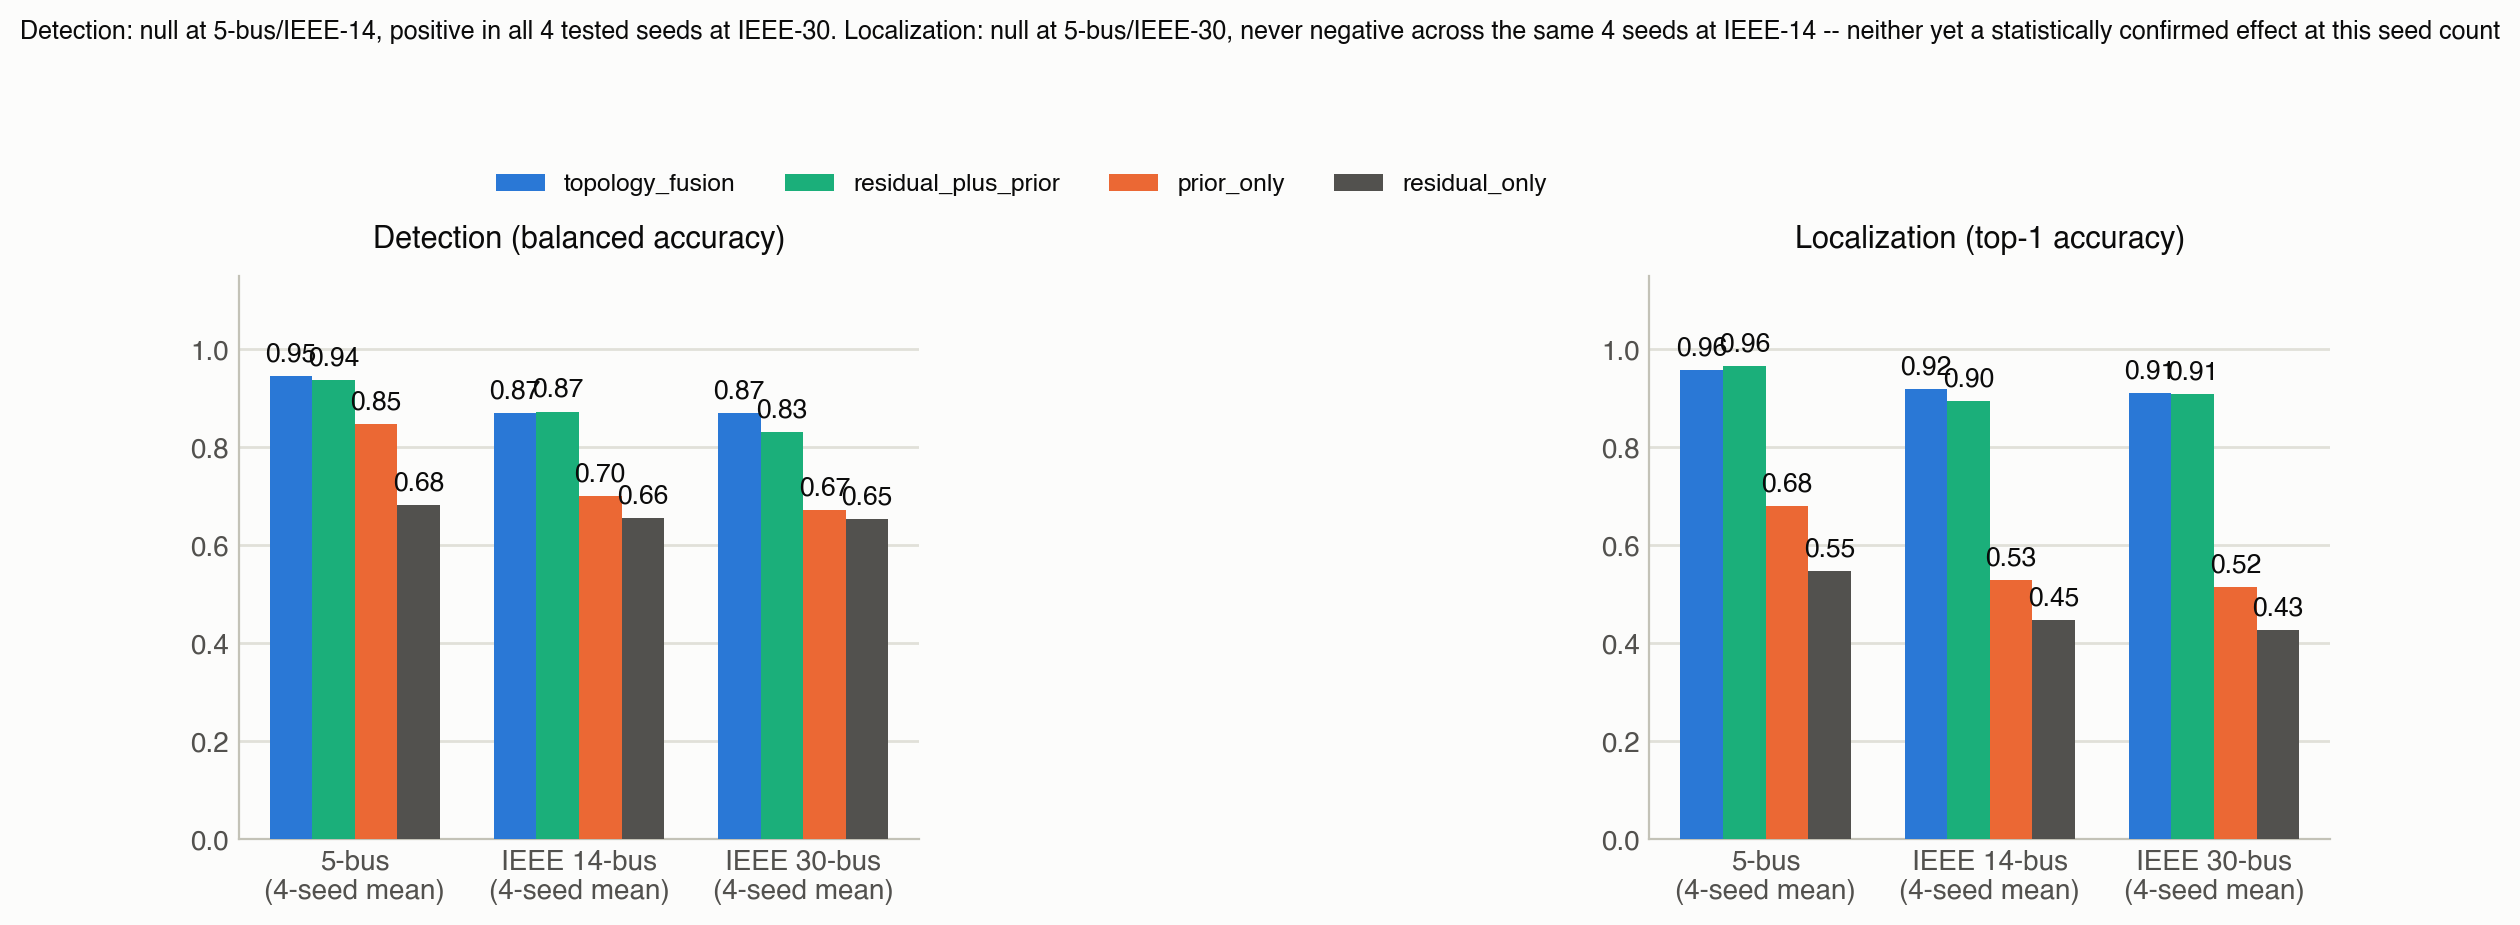
\includegraphics[width=\columnwidth]{paper_fig4_scale_comparison.png}
\caption{5-bus vs.\ IEEE 14-bus vs.\ IEEE 30-bus, all 4-seed means, all four feature sets. Detection: null at 5-bus/IEEE-14, positive in all 4 tested seeds at IEEE-30. Localization: null at 5-bus/IEEE-30, never negative across the same 4 seeds at IEEE-14. Each task's consistent-sign gap, where one exists, is specific to one network, not shared between the two standard IEEE systems and never present at the custom microgrid; neither is yet a statistically confirmed effect at this seed count (Section~\ref{sec:scale}).}
\label{fig:scale}
\end{figure}

\begin{table}[t]
\centering
\caption{IEEE 14-bus, \texttt{topology\_fusion} vs.\ the best non-relational alternative each seed, 4 independent seeds (500 repl.\ each)}
\label{tab:ieee14seeds}
\footnotesize
\begin{tabular}{@{}ccc@{}}
\toprule
Seed & Detection gap & Localization gap \\
\midrule
20260921 & $-0.013$ & $+0.000$ \\
42 & $-0.013$ & $+0.047$ \\
777 & $-0.000$ & $+0.033$ \\
2024 & $+0.014$ & $+0.013$ \\
\midrule
mean $\pm$ std & $-0.003 \pm 0.013$ & $+0.023 \pm 0.021$ \\
\bottomrule
\end{tabular}
\end{table}

\begin{table}[t]
\centering
\caption{IEEE 30-bus, \texttt{topology\_fusion} vs.\ the best non-relational alternative each seed, 4 independent seeds (500 repl.\ each)}
\label{tab:ieee30seeds}
\footnotesize
\begin{tabular}{@{}ccc@{}}
\toprule
Seed & Detection gap & Localization gap \\
\midrule
20260921 & $+0.080$ & $-0.020$ \\
42 & $+0.040$ & $-0.007$ \\
777 & $+0.023$ & $+0.000$ \\
2024 & $+0.013$ & $+0.033$ \\
\midrule
mean $\pm$ std & $+0.039 \pm 0.029$ & $+0.002 \pm 0.023$ \\
\bottomrule
\end{tabular}
\end{table}

\subsection{Cross-Network Result}
At IEEE 14-bus (Table~\ref{tab:ieee14seeds}), the detection gap changes sign across seeds ($-0.013$ to $+0.014$, mean $-0.003\pm0.013$) -- null, matching 5-bus. The localization gap does not: non-negative in all 4 seeds ($+0.000$ to $+0.047$, mean $+0.023\pm0.021$, three seeds strictly positive and one exact tie), never favoring the non-relational alternative. At IEEE 30-bus (Table~\ref{tab:ieee30seeds}), the pattern inverts entirely: the detection gap is positive in all 4 seeds ($+0.013$ to $+0.080$, mean $+0.039\pm0.029$) -- roughly 1.7$\times$ IEEE-14's localization effect. The localization gap at IEEE-30 changes sign across seeds ($-0.020$ to $+0.033$, mean $+0.002\pm0.023$) -- null, matching 5-bus.

\subsection{Statistical Caveat}
With four seeds, the observed sign consistency can be reported, but the sample is not sufficient on its own to call an effect statistically confirmed. A standard $t$-based 95\% confidence interval on the IEEE-30 detection gap is $+0.039 \pm 0.047$ (i.e.\ $[-0.008, 0.086]$), and on the IEEE-14 localization gap is $+0.023 \pm 0.033$ (i.e.\ $[-0.010, 0.056]$) -- both cross zero. A distribution-free sign test gives a one-sided $p=0.5^4=0.0625$ for the IEEE-30 detection gap (four of four seeds strictly positive); the IEEE-14 localization gap includes one exact tie (Table~\ref{tab:ieee14seeds}), which a sign test conventionally excludes rather than counts as a positive, leaving three of three non-zero seeds positive and $p=0.5^3=0.125$ -- weaker evidence than IEEE-30's, not the same figure. Neither reaches the conventional 0.05 threshold. We therefore describe both findings throughout this paper as \emph{consistent in sign across all four tested seeds}, not as a statistically confirmed effect: the evidence is that every seed drawn so far points the same way (or ties, never against it), which is meaningfully different from, and weaker than, a claim that the underlying effect is confirmed nonzero. The sign test's own bar is low if the pattern holds -- a fifth same-direction seed at IEEE-30 would already cross one-sided $p<0.05$ ($0.5^5=0.03125$) -- so the 10--20-seed estimate below targets a harder goal instead: a tight confidence interval on the effect's \emph{magnitude}, not sign-test significance. Resolving that would require additional seeds or a paired/bootstrap difference test; neither is included here, so the effect is reported as sign-consistent rather than statistically confirmed.

\subsection{Interpretation}
Across the three networks and two tasks, the result is: \emph{detection} shows no reproducible topology advantage at 5-bus or IEEE-14, but a consistent-sign one at IEEE-30; \emph{localization} shows no reproducible advantage at 5-bus or IEEE-30, but a consistent-sign one at IEEE-14 (four tested seeds each, neither yet a statistically confirmed effect on its own -- Section~\ref{sec:scale}'s explicit caveat). Neither task is uniform across networks, and the two consistent-sign gaps do not co-occur at the same network; the observed pattern is therefore incompatible with a simple network-independent rule for when explicit topology features help. This is consistent with, and sharpens, a 2025 field-wide scoping review's \cite{oelhaf2025scoping} independent finding that cross-topology generalization is essentially untested across the ML-for-power-protection literature it surveyed -- this study is a direct, sample-size-matched, cross-implementation attempt at a gap the field has already named.

\section{Discussion}

Read together, Sections~\ref{sec:results1}--\ref{sec:scale} converge on a finding that is uniform for neither task, reached across three networks and two independently implemented feature pipelines. For \emph{detection}: explicit topology-relational features show no reproducible advantage over a matched non-relational ablation at 5-bus (a null, sign-unstable gap, mean $+0.008\pm0.012$) or IEEE 14-bus (a null, sign-unstable gap, mean $-0.003\pm0.013$) -- but a gap positive in all four tested seeds at IEEE 30-bus (mean $+0.039\pm0.029$). For \emph{localization}: no reproducible advantage at 5-bus (a null, sign-unstable gap, mean $-0.007\pm0.016$, after removing degree/role metadata) or IEEE 30-bus (a null, sign-unstable gap) -- but a gap never negative across the same four seeds at IEEE 14-bus (mean $+0.023\pm0.021$). Put plainly: each of the two standard IEEE test systems shows a topology-favoring gap that holds its sign across all four tested seeds in exactly one of the two tasks, and it is a \emph{different} task at each network; the small custom 5-bus microgrid shows no such gap in either task. As Section~\ref{sec:scale} states explicitly, four same-signed seeds is consistent-sign evidence, not a statistically confirmed effect -- a $t$-based confidence interval at this sample size crosses zero for both gaps, and neither should be read as more settled than that.

What helps detection at 5-bus, considerably, is combining residual and prior-innovation information: a consistent multi-seed gain over either source alone (Section~\ref{sec:results1}) -- not a topology-specific effect. Section~\ref{sec:results1}'s redundancy analysis gives the 5-bus null results (now on both tasks) a structural, not just empirical, footing: on a fixed, small topology, a relational aggregate is close to a linear function of information a flexible classifier already has (mean out-of-fold $R^2 = 0.956$), so there is little left for an explicit relational feature to contribute. A natural hypothesis is that this redundancy weakens on a larger, more meshed network, potentially explaining the IEEE-14 localization result. The same diagnostic was therefore applied to IEEE-14's relational localization features (each node's neighbor-mean/-max and local-minus-neighbor values, predicted from all 14 nodes' local residual/innovation values) gives a mean $R^2$ of 0.966 (median 0.999, 92\% of columns above 0.8) -- if anything \emph{higher} than the 5-bus figure, not lower. Reduced linear recoverability does not explain the IEEE-14 localization pattern under this diagnostic. We have not run the equivalent check for IEEE-30's detection-relevant relational features -- unlike the localization case, where the same node-level check design transfers directly between 5-bus and IEEE-14, IEEE-30's detection features and 5-bus's use different, non-comparable representations, and building a third variant of this diagnostic was judged out of scope here; whether redundancy explains IEEE-30's detection pattern remains an open question.

One plausible explanation for the IEEE-14 case, though not directly verified, is discoverability rather than availability: HistGradientBoosting -- a tree-based model with no built-in notion of ``neighbor'' -- must find the right subset of a flat, unstructured input to combine for each target node, a search that may be harder with more nodes even when the information needed is linearly present throughout; being handed the relational feature directly removes that search entirely. This remains a genuine open question this paper raises rather than resolves, and the picture is now more complicated than a single ``does discoverability get harder with scale'' story would predict: IEEE-30 is larger than IEEE-14 by node count, yet its \emph{localization} redundancy-driven story (if that is what IEEE-14's is) does not extend to it at all -- IEEE-30's own localization gap is null -- while IEEE-30 instead shows an advantage in the \emph{other} task, detection, which 5-bus and IEEE-14 both show no advantage in. A mechanism that predicts discoverability difficulty scaling smoothly with network size, uniformly across tasks, does not fit this pattern; a mechanism that is specific to some other property of each network (redundancy in exactly which quantities, exactly how the attack and measurement models interact with each network's own topology) might, but identifying that property is future work, not something this paper's evidence settles.

The more important finding here is not a scale boundary on a single confirmed effect, but a genuinely task- and network-specific pattern with two distinct, consistent-sign gaps and no uniform story connecting them.

\section{Limitations}

\begin{enumerate}
\item \textbf{Scale and network-specificity}: Three network topologies have now been tested to the same 4-seed standard. Detection shows a gap consistently positive across all four tested seeds at exactly one of them (IEEE-30); localization at exactly one, different, network (IEEE-14), never negative across the same four seeds. None uses a real (non-synthetic) network or load profile, and with only three networks tested, the emerging pattern (each standard IEEE system favoring a different task) is a two-data-point observation, not something a fourth or fifth network is guaranteed to extend in either direction.
\item \textbf{Four seeds is consistent-sign evidence, not a statistically confirmed effect}: both surviving gaps (IEEE-30 detection, IEEE-14 localization) are positive/non-negative in all four tested seeds, but a standard $t$-based 95\% confidence interval crosses zero for both ($+0.039\pm0.047$ and $+0.023\pm0.033$ respectively). A distribution-free sign test does not reach $p<0.05$ for either: one-sided $p=0.0625$ for IEEE-30 (four of four seeds positive), and $p=0.125$ for IEEE-14 once its one exact tie is excluded per sign-test convention (three of three non-zero seeds positive, not four of four). We describe both findings as consistent in sign across every seed tested, deliberately short of claiming statistical confirmation; one further same-direction seed would cross the sign test's own 0.05 threshold at IEEE-30, but a stable estimate of either effect's magnitude would need roughly 10--20 seeds or a paired/bootstrap difference test, neither run here.
\item \textbf{Cross-network measurement-noise and forecast-uncertainty mismatch}: measurement standard deviations are fixed absolute values shared, unscaled, across all three networks despite their very different physical scales, and prior load-forecast uncertainty is 2.5\% at 5-bus vs.\ 5\% at IEEE-14/IEEE-30 (Section~\ref{sec:method}). This was not standardized or swept as an independent robustness axis; the cross-network comparisons in Section~\ref{sec:scale} should be read with this confound explicitly in mind, not as a controlled scale-only experiment. In light of this, ``network-specific'' throughout this paper is more precisely \emph{setup-and-network-specific under the tested measurement/prior regimes}: each network's result reflects its topology together with its own noise/prior configuration, not topology in isolation. IEEE-14 and IEEE-30 share an identical noise/prior convention, so their disagreement with each other (one task's gap each, not the same task) is not subject to this particular confound; only comparisons that include 5-bus are.
\item \textbf{No zero-day generalization} (Section~\ref{sec:zeroday}): detection/localization numbers hold only for attack types represented in training -- verified for both \texttt{topology\_fusion} and \texttt{residual\_plus\_prior}, which collapse identically (Table~\ref{tab:zeroday}), under a corrected, symmetric evaluation protocol; localization was not separately re-tested for zero-day generalization (only detection was), and the underlying attack taxonomy is still limited to two families (item 5 below).
\item \textbf{Single testbed family, two attack types}: the present AC-consistent attack generator does not independently vary the compromised-measurement subset; introducing explicit attacker-access constraints (e.g.\ a fixed budget of compromisable sensors) as a separate, tunable threat-model parameter is left for future work.
\item \textbf{Latency results} (Section~\ref{sec:latency}) characterize one documented Apple-arm64/macOS 15.6.1 Python/\texttt{pandapower} environment, not a hardware or RTOS claim, and were not re-benchmarked on the smaller \texttt{residual\_plus\_prior} feature set (Section~\ref{sec:latency} argues this would not change the conclusion, since state estimation, not classification, dominates the budget, but this is an argument, not a re-measurement).
\end{enumerate}

\section{Conclusion}

Across a small custom inverter-dominated microgrid and two standard, larger IEEE test systems (14-bus and 30-bus), explicit topology-relational features show no uniform advantage for either detection or localization. What they show instead is a strictly task-and-network-specific pattern: a detection gap consistently positive across all four tested seeds at IEEE 30-bus only (never at 5-bus or IEEE 14-bus), and a localization gap never negative across the same four seeds at IEEE 14-bus only (never at 5-bus or IEEE 30-bus) -- both, we state explicitly, consistent-sign evidence rather than a statistically confirmed effect: a 4-seed confidence interval crosses zero for either gap on its own, and resolving that properly would need substantially more seeds than this paper reports. We take this as a caution against generalizing any single network's result -- in either direction, for either task -- into a general rule from one or two data points. Separately, the resulting decision pipeline, verified with a trained classifier and deployable features throughout, can be brought within a one-cycle target once its actual bottleneck, a software inefficiency, is fixed, and the detector does not extend to attack types unseen in training.


\bibliographystyle{IEEEtran}
\bibliography{references}

\end{document}
